\documentclass{article}
	\usepackage[utf8]{inputenc}
	\usepackage{float}
	\usepackage{pdfpages}
	\usepackage[T1]{fontenc}
	\usepackage{float}
	\usepackage{booktabs}
	\usepackage{multirow}
	\usepackage{ragged2e}
	\usepackage{makecell}
	\renewcommand{\theadfont}{\small\bfseries}
	\usepackage{tabularx}
	\usepackage[autolanguage, np]{numprint}
	\newcolumntype{Z}{ >{\centering\arraybackslash}X }
	\usepackage{makecell}
	\usepackage{url}
	\usepackage{siunitx}
	\usepackage{caption}
	\usepackage[framemethod=TikZ]{mdframed}
	\usepackage{tikz, tabularx}
	\usepackage[T1]{fontenc}
	\usepackage{charter}

%%% Document Properties and Packages used 9/20
\usepackage{amsmath}        % math formulas
\usepackage{bm}             % bold math symbols
\usepackage{multicol}       % multiple columns
\usepackage[super]{nth}     % 1st, 2nd, 3rd, 4th
\usepackage{enumitem}       % ordered list (a), (b), (c)
\usepackage{graphicx}		% insert images
\graphicspath{ {./images/} }
\usepackage{geometry}
\geometry{letterpaper, margin=1in, top=0.5in} % small margins
\usepackage{biblatex}		% bibliography
\addbibresource{HW1N1.bib}
%%%%%%%%%%%%%%%%%%%%%%%%%%%%%%%%%%%%%%%%%%%%%%%%%%%%%%%%%%%%%%%%%%%%%%%%%%%%%%%
%%% Code Listing 
\usepackage{listings}
\usepackage{xcolor}

\definecolor{codegreen}{rgb}{0,0.6,0}
\definecolor{codegray}{rgb}{0.5,0.5,0.5}
\definecolor{codepurple}{rgb}{0.58,0,0.82}
\definecolor{backcolour}{rgb}{0.95,0.95,0.92}

\lstdefinestyle{mystyle}{
	backgroundcolor=\color{backcolour},   
	commentstyle=\color{codegreen},
	keywordstyle=\color{magenta},
	numberstyle=\tiny\color{codegray},
	stringstyle=\color{codepurple},
	basicstyle=\ttfamily\footnotesize,
	breakatwhitespace=false,         
	breaklines=true,                 
	captionpos=b,                    
	keepspaces=true,                 
	numbers=left,                    
	numbersep=5pt,                  
	showspaces=false,                
	showstringspaces=false,
	showtabs=false,                  
	tabsize=2
}
\lstset{style=mystyle}
%%%%%%%%%%%%%%%%%%%%%%%%%%%%%%%%%%%%%%%%%%%%%%%%%%%%%%%%%%%%%%%%%%%%%%%%%%%%%%%
\begin{document}
	
	\noindent\textbf{Justine John "JJ" A. Serdoncillo}
	\hfill \textbf{AEM 8202: Fluid Mechanics 2} \\ \hfill \textbf{February 28, 2023}
	
	\begin{center}
		\Large{\textbf{Homework 2}}    
	\end{center}
	
	\section*{Number 1 c)}
		After determining the necessary complex potential function for this flow, the streamlines and potential lines are plotted as seen in the figure below. The solid lines correspond to the streamlines while the dashed, translucent lines correspond to the potential lines. The red points are the stagnation points and it can be seen that it does lie on the following required locations. The black arrows are the quiver plot for the velocity flow. 

		\begin{figure}[H]
			\centering
			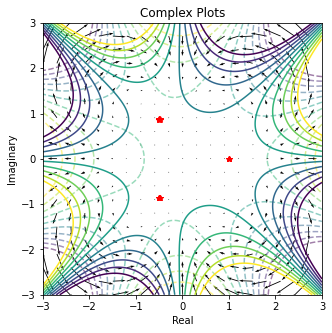
\includegraphics[width=0.6\textwidth]{images/first.png}
			\caption{ Complex Potential Flow for 3 Stagnation Points}
		\end{figure}
	
	\section*{Number 2 a)}
		After determining the necessary complex potential function for this flow, the streamlines are plotted as seen in the figure below. Similarly, the potential lines are also plotted as dashed translucent lines. It can be seen that the flow is acting on a flat plate and this is done using the method of images. 
		
		\begin{figure}[H]
			\centering
			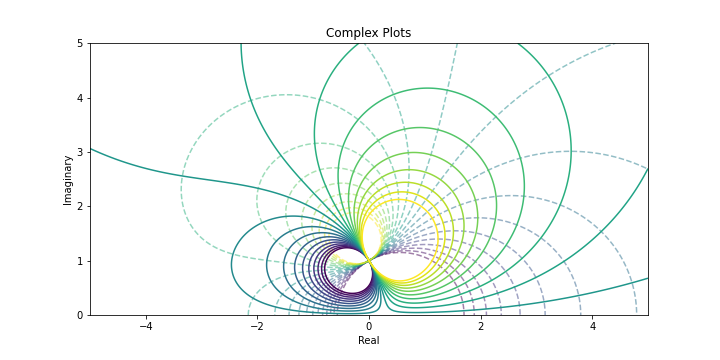
\includegraphics[width=1\textwidth]{images/second.png}
			\caption{ Complex Potential Flow for Dipole on Infinite Flat Plate}
		\end{figure}
		
	\section*{Number 3 d}
		The following streamlines are plotted for the two elliptical flows. The blue dots correspond to points that evaluate to the 0 streamline, while the cyan lines are with the 17cm streamline. It can be seen that at x=0, the cyan line is at around 60 which corresponds to the similar htop calculated of 11.67cm. The same can be said for the Prized Rose problem showing a smaller htop of around 3.33cm.
		
		\begin{figure}[H]
			\centering
			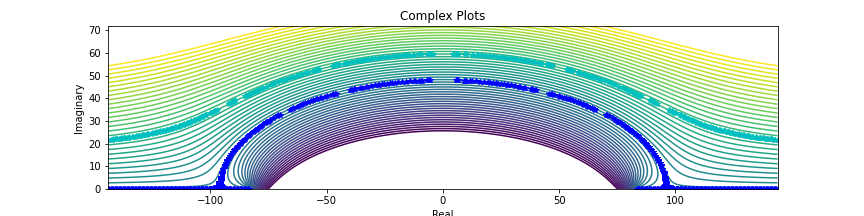
\includegraphics[width=1\textwidth]{images/third.png}
			\caption{ Streamlines for Elliptic Greenhouse}
		\end{figure}

		\begin{figure}[H]
			\centering
			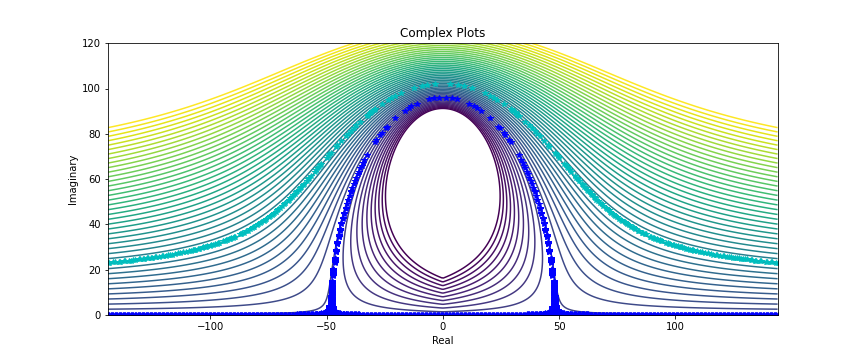
\includegraphics[width=1\textwidth]{images/fourth.png}
			\caption{ Streamlines for Elliptic Prized Rose}
		\end{figure}
		
		Using the BEM solver from the previous homework, the following figures are created as shown below. 
		
		\begin{figure}[H]
			\centering
			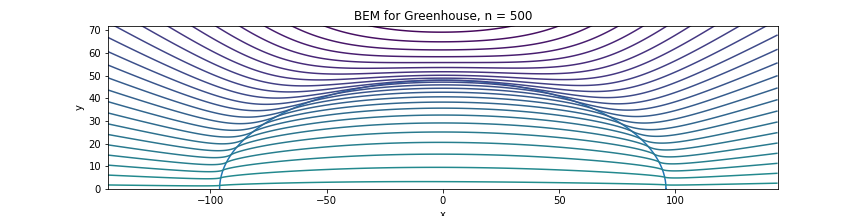
\includegraphics[width=1\textwidth]{images/BEM1.png}
			\caption{ Streamlines from BEM Solver for Greenhouse}
		\end{figure}
	
		\begin{figure}[H]
			\centering
			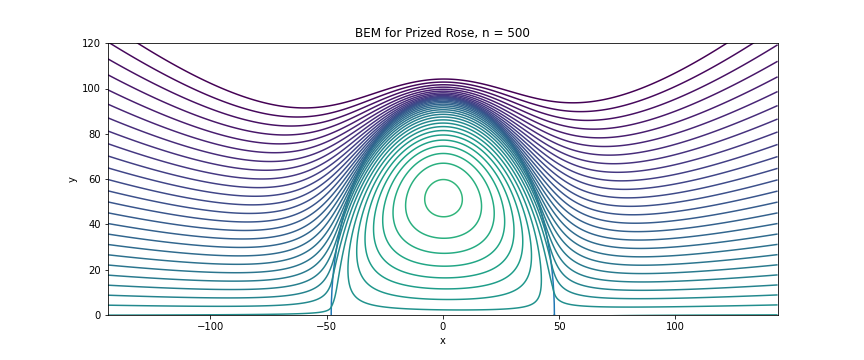
\includegraphics[width=1\textwidth]{images/BEM2.png}
			\caption{ Streamlines from BEM Solver for Prized Rose}
		\end{figure}
	
		It can be seen that there is a clear difference between the analytical solution and the BEM method. It can be seen that from using the BEM method, the streamlines are somewhat going up instead of going down. At close streamlines to the surface this may be an accurate representation, however, close to infinity, it doesn't show a proper uniform flow. 
		
		\newpage
		\section*{Appendix)}
			\subsection*{ Python Code for Problems 1,2,3 }
			\lstinputlisting[language=Python]{HW2_v4_4_formating.py}
			\newpage
			\subsection*{ Python Code for Problem 3 BEM Solver }
			\lstinputlisting[language=Python]{HW2P3c_v3_formatting.py}
			
			
	
	
\end{document}
